% Template for PLoS
% Version 3.3 June 2016
%
% % % % % % % % % % % % % % % % % % % % % %
%
% -- IMPORTANT NOTE
%
% This template contains comments intended 
% to minimize problems and delays during our production 
% process. Please follow the template instructions
% whenever possible.
%
% % % % % % % % % % % % % % % % % % % % % % % 
%
% Once your paper is accepted for publication, 
% PLEASE REMOVE ALL TRACKED CHANGES in this file 
% and leave only the final text of your manuscript. 
% PLOS recommends the use of latexdiff to track changes during review, as this will help to maintain a clean tex file.
% Visit https://www.ctan.org/pkg/latexdiff?lang=en for info or contact us at latex@plos.org.
%
%
% There are no restrictions on package use within the LaTeX files except that 
% no packages listed in the template may be deleted.
%
% Please do not include colors or graphics in the text.
%
% The manuscript LaTeX source should be contained within a single file (do not use \input, \externaldocument, or similar commands).
%
% % % % % % % % % % % % % % % % % % % % % % %
%
% -- FIGURES AND TABLES
%
% Please include tables/figure captions directly after the paragraph where they are first cited in the text.
%
% DO NOT INCLUDE GRAPHICS IN YOUR MANUSCRIPT
% - Figures should be uploaded separately from your manuscript file. 
% - Figures generated using LaTeX should be extracted and removed from the PDF before submission. 
% - Figures containing multiple panels/subfigures must be combined into one image file before submission.
% For figure citations, please use "Fig" instead of "Figure".
% See http://journals.plos.org/plosone/s/figures for PLOS figure guidelines.
%
% Tables should be cell-based and may not contain:
% - spacing/line breaks within cells to alter layout or alignment
% - do not nest tabular environments (no tabular environments within tabular environments)
% - no graphics or colored text (cell background color/shading OK)
% See http://journals.plos.org/plosone/s/tables for table guidelines.
%
% For tables that exceed the width of the text column, use the adjustwidth environment as illustrated in the example table in text below.
%
% % % % % % % % % % % % % % % % % % % % % % % %
%
% -- EQUATIONS, MATH SYMBOLS, SUBSCRIPTS, AND SUPERSCRIPTS
%
% IMPORTANT
% Below are a few tips to help format your equations and other special characters according to our specifications. For more tips to help reduce the possibility of formatting errors during conversion, please see our LaTeX guidelines at http://journals.plos.org/plosone/s/latex
%
% For inline equations, please be sure to include all portions of an equation in the math environment.  For example, x$^2$ is incorrect; this should be formatted as $x^2$ (or $\mathrm{x}^2$ if the romanized font is desired).
%
% Do not include text that is not math in the math environment. For example, CO2 should be written as CO\textsubscript{2} instead of CO$_2$.
%
% Please add line breaks to long display equations when possible in order to fit size of the column. 
%
% For inline equations, please do not include punctuation (commas, etc) within the math environment unless this is part of the equation.
%
% When adding superscript or subscripts outside of brackets/braces, please group using {}.  For example, change "[U(D,E,\gamma)]^2" to "{[U(D,E,\gamma)]}^2". 
%
% Do not use \cal for caligraphic font.  Instead, use \mathcal{}
%
% % % % % % % % % % % % % % % % % % % % % % % % 
%
% Please contact latex@plos.org with any questions.
%
% % % % % % % % % % % % % % % % % % % % % % % %

\documentclass[10pt,letterpaper]{article}
\usepackage[top=0.85in,left=2.75in,footskip=0.75in]{geometry}

% amsmath and amssymb packages, useful for mathematical formulas and symbols
\usepackage{amsmath,amssymb}

% Use adjustwidth environment to exceed column width (see example table in text)
\usepackage{changepage}

% Use Unicode characters when possible
\usepackage[utf8x]{inputenc}

% textcomp package and marvosym package for additional characters
\usepackage{textcomp,marvosym}

% cite package, to clean up citations in the main text. Do not remove.
\usepackage{cite}

% Use nameref to cite supporting information files (see Supporting Information section for more info)
\usepackage{nameref,hyperref}

% line numbers
\usepackage[right]{lineno}

% ligatures disabled
\usepackage{microtype}
\DisableLigatures[f]{encoding = *, family = * }

% color can be used to apply background shading to table cells only
\usepackage[table]{xcolor}

% array package and thick rules for tables
\usepackage{array}

\usepackage{csquotes}

% create "+" rule type for thick vertical lines
\newcolumntype{+}{!{\vrule width 2pt}}

% create \thickcline for thick horizontal lines of variable length
\newlength\savedwidth
\newcommand\thickcline[1]{%
  \noalign{\global\savedwidth\arrayrulewidth\global\arrayrulewidth 2pt}%
  \cline{#1}%
  \noalign{\vskip\arrayrulewidth}%
  \noalign{\global\arrayrulewidth\savedwidth}%
}

% \thickhline command for thick horizontal lines that span the table
\newcommand\thickhline{\noalign{\global\savedwidth\arrayrulewidth\global\arrayrulewidth 2pt}%
\hline
\noalign{\global\arrayrulewidth\savedwidth}}


% Remove comment for double spacing
%\usepackage{setspace} 
%\doublespacing

% Text layout
\raggedright
\setlength{\parindent}{0.5cm}
\textwidth 5.25in 
\textheight 8.75in

% Bold the 'Figure #' in the caption and separate it from the title/caption with a period
% Captions will be left justified
\usepackage[aboveskip=1pt,labelfont=bf,labelsep=period,justification=raggedright,singlelinecheck=off]{caption}
\renewcommand{\figurename}{Fig}

% Use the PLoS provided BiBTeX style
\bibliographystyle{plos2015}

% Remove brackets from numbering in List of References
\makeatletter
\renewcommand{\@biblabel}[1]{\quad#1.}
\makeatother

% Leave date blank
\date{}

% Header and Footer with logo
\usepackage{lastpage,fancyhdr,graphicx}
\usepackage{epstopdf}
\pagestyle{myheadings}
\pagestyle{fancy}
\fancyhf{}
\setlength{\headheight}{27.023pt}
\lhead{
\includegraphics[width=2.0in]{PLOS-submission.eps}}
\rfoot{\thepage/\pageref{LastPage}}
\renewcommand{\footrule}{\hrule height 2pt \vspace{2mm}}
\fancyheadoffset[L]{2.25in}
\fancyfootoffset[L]{2.25in}
\lfoot{\sf PLOS}

%% Include all macros below

\newcommand{\lorem}{{\bf LOREM}}
\newcommand{\ipsum}{{\bf IPSUM}}

%% END MACROS SECTION


\begin{document}
\vspace*{0.2in}

% Title must be 250 characters or less.
\begin{flushleft}
{\Large
\textbf\newline{Microvessel Chaste: A Library for Multi-Scale Agent-Based Simulation of Tissues with Microvessels} % Please use "title case" (capitalize all terms in the title except conjunctions, prepositions, and articles).
}
\newline
% Insert author names, affiliations and corresponding author email (do not include titles, positions, or degrees).
\\
James A. Grogan\textsuperscript{1*},
Anthony J. Connor\textsuperscript{1, 2},
Philip K. Maini\textsuperscript{1},
Helen M. Byrne\textsuperscript{1},
Joe Pitt-Francis\textsuperscript{2}
\\
\bigskip
\textbf{1} Wolfson Centre for Mathematical Biology, Mathematical Institute, University of Oxford, Oxford, \mbox{OX2 6GG}, UK.
\\
\textbf{2} Department of Computer Science, University of Oxford, Oxford, \mbox{OX1 3QD}, UK.
\\
\bigskip

% Insert additional author notes using the symbols described below. Insert symbol callouts after author names as necessary.
% 
% Remove or comment out the author notes below if they aren't used.
%
% Primary Equal Contribution Note
%\Yinyang These authors contributed equally to this work.

% Additional Equal Contribution Note
% Also use this double-dagger symbol for special authorship notes, such as senior authorship.
%\ddag These authors also contributed equally to this work.

% Current address notes
%\textcurrency Current Address: Dept/Program/Center, Institution Name, %City, State, Country % change symbol to "\textcurrency a" if more than one current address note
% \textcurrency b Insert second current address 
% \textcurrency c Insert third current address

% Deceased author note
%\dag Deceased

% Group/Consortium Author Note
%\textpilcrow Membership list can be found in the Acknowledgments section.

% Use the asterisk to denote corresponding authorship and provide email address in note below.
* grogan@maths.ox.ac.uk

\end{flushleft}
% Please keep the abstract below 300 words
\section*{Abstract}
Microvessel Chaste is an open-source software library for multi-scale agent-based modelling of tissues with microvessels. Development has focused on applications in spatial modelling of vascular tumours and wound healing. Problems of interest in these areas involve modelling blood flow, temporally evolving vessel network geometries and topologies and vessel interactions with diffusible chemicals. This library integrates discrete representations of microvessels with already re-usable components for agent-based modelling in Chaste, such as discrete cells, meshes and ordinary and partial differential equation (ODE/PDE) solvers. The aims of the library are to facilitate i) rapid model composition from a range of interchangeable sub-models, ii) management of a large number of input parameters from heterogenous literature sources and iii) integration of modelling with experimental observations. These aims are pertinent in the area of discrete vascular tissue modelling, where model cross-comparison and experimental validation are still in early stages. This article includes simple example applications of the library which can be run on a desktop computer. The source code is available to download under an open source Berkeley Software Distribution (BSD) licence at \url{https://chaste.cs.ox.ac.uk/trac/wiki/PaperTutorials/Microvessel}, together with details of a mailing list [JG: add mailing list info to landing page] and links to documentation and tutorials.

\linenumbers

% Use "Eq" instead of "Equation" for equation citations.
\section*{Introduction}
Cancer, Heart And Soft Tissue Environment (Chaste) is an open-source C++ library which has been developed to enable the study of problems in computational physiology and biology. As discussed in a dedicated article~\cite{Mirams2013}, the library has been designed with a focus on: i) facilitating the rapid development of computational models and methods through code re-use and documentation and ii) overcoming challenges related to the reliability and reproducbility of computational results. Chaste has been widely used in cardiac electrophysiology~\cite{Cooper2015}, developmental biology~\cite{Tetley2016} and cancer applications~\cite{Dunn2016}. While some applications have focused on tumour modelling~\cite{Figueredo2013}, the library does not have functionality for modelling microvessels. Chaste allows for the development of 'add-on' projects which share the same build system and documentation tools. Microvessel Chaste is an add-on project with functionality for discrete modelling of microvessels.

Multi-scale agent-based modelling of tissue with microvessels, as applied in studying vascular tumours~\cite{Owen2011}, introduces several requirements beyond those faced by dedicated cell modelling software, notible examples of which are CompuCell3D~\cite{Swat2012}, EPISIM~\cite{Sutterlin2013} and PhysiCell~\cite{Macklin2012}. For example, i) line or surface based representations of vessels are needed in place of point or centre-based representations of cells, ii) blood flow and chemical transport problems are solved in vessel networks with constantly evolving vessel geometry and connectivity and iii) new vessels may form and migrate based on mechanical and chemical cues. These requirements are additional to those of cell-only frameworks, such as cell-cycling, migration, proliferation and interaction with diffusible chemicals. Models of this type typically use a relatively large number of input parameters (over 100 in Owen et al.~\cite{Owen2011}) from heterogeneous literature sources. In addition, there is a variety of ways in which a model can be composed from interchangeable sub-models, with interchangeable solution ordering. Development of Microvessel Chaste aims to implement the additional requirements for multi-scale agent-based modelling of tissue with microvessels, while adhering to the original Chaste Project design goals. This is done by focusing on i) \emph{extensibility}, ii) \emph{documentation}, iii) \emph{reproducibility} and iv) \emph{efficiency} of both models and code through the use of object oriented design, C++ for computational efficiency, and Boost Units~\cite{boost161} for compile-time dimensional analysis. 

To the authors' knowledge there is currently no dedicated software framework for composing multi-scale agent-based models of tissue microvascaulture of the type in~\cite{Owen2011}. While the are many notable bespoke computational models of tissue microvascaulture, including Secomb et al.~\cite{Secomb2013}, Anderson and Chaplain~\cite{Anderson1998}, Friboes et al.~\cite{Frieboes2007}, Shirinifard et al.~\cite{Shirinifard2009} and Welter and Rieger~\cite{Welter2013}, the resulting software does not meet all of the following desirable attributes, i) availability under a permissive open source license, ii) API documentation and user tutorials, iii) capability for on- and off-lattice modelling of vessels in arbitary geometries in two and three dimensions and iv) use of object-oreinted design. These attributes are the focus of Microvessel Chaste.

The mentioned attributes allow utilization of the library in addressing two outstanding challenges in tissue microvascaulture modelling. \emph{First}, the importance of rapidly constructing and cross-comparing multi-scale agent-based models of tissue microvascaulture is well recognized, as are the challenges in developeing software for such an endeavour~\cite{Rieger2015, Connor2012}. One hurdle which the library helps overcome is the lack of open-source, documented software in the field. This has previously made it neccessary to re-implement each computational model before application, delaying comparison studies. While the present authors have previously developed and applied a range of multi-scale agent-based microvessel models in the areas of cancer~\cite{Alarcon2005, Perfahl2011} and angiogenesis~\cite{Connor2015}, their incorporation in Microvessel Chaste is the first time such models have been made available open-source, with documentation and tutorials. \emph{Second}, there is now a wealth of high resolution three-dimensional experimental imaging data against which model predictions can be compared~\cite{Tozer2004}. To fully exploit this data it is neccessary that three-dimensional tissue regions of resonable volume with realistic geometries can be simulated, as per~\cite{Grogan2016}. There are few approaches developed for this purpose in the literature. Such functionality is availble in the Microvessel Chaste library, including previously unpublished methods for three-dimensional off-lattice modelling of sprouting angiogenesis.  

This article accompanies the first release of the Microvessel Chaste library, although some elements have been used in previous studies~\cite{Connor2015, Grogan2016}. Code design and implementation are discussed in the next section, followed by a collection of simple sample applications. The sample applications are design to be quickly run on a desktop PC, in practice more expensive simulations are usually performed. Examples can be run and figures re-created by downloading the project from \url{https://chaste.cs.ox.ac.uk/trac/wiki/PaperTutorials/Microvessel}. 

\section*{Design and Implementation}

This section briefly summarizes available algorithms by demonstrating how the library may be used to construct and solve a typical multi-scale agent-based microvessel problem. A dedicated article should be consulted for further details on algorithms related to core Chaste functionality, such as linear algebra, input/output, and discrete cell modelling~\cite{Mirams2013}. It is noted that development of the MicroVessel Chaste library has not strictly followed the Test-Driven Development and Agile-Programming practices adopted by the Chaste Project, although it aims for full unit-test and API documentation code coverage. The library can be used with Linux only, with virtual machines required for use on Microsoft Windows and Mac OS X. The C++ interface requires building from source after downloading and setting up dependencies, which can up to an hour the first time.

\subsection*{Algorithm Overivew}

The library is designed for composing multi-scale agent-based problems for tissue with microvessels using on- and off-lattice representations of cells and vessels. While the library attempts to minimize the imposition of a definitive model structure on the user, it is helpful when introducing algorithms to consider a concentre use case. 

Fig~\ref{fig1} shows how the library can be used to \emph{compose} a problem of interest in vascular tumour modelling. For further details on models of this type the reader can refer to Alarcon et al.~\cite{Alarcon2005} and Owen et al.~\cite{Owen2011}. In this example, an initial vessel network and cell population are constructed, transport PDEs for diffusible chemicals defined, rules for vessel growth or shrinkage due to blood flow defined, along with rules for vessel sprouting and endothelial tip cell migration in a stimulus field. The ability to compose a model from a collection of sub-models and sub-sub models is noted. Models and sub-models can be over-ridden by the user with both C++ and Python frameworks, which is useful for implenting custom migration and sprouting rules, for example. It is noted that there is a high degree of interaction between components. Once a domain, which is a geometrical feature in 2D or 3D, is defined it can be used in the construction of vessel networks and cell populations through multiple space-filling or boolean operations, and in the generation of a computational grid (mesh) for use in the solution of PDEs. Similarly, once vessel networks and cell populations have been defined they can be passed as objects (via shared pointers) to other components, allowing the definition of boundary conditions or PDE sinks and sources which depend on vessel and cell locations. Sub-models can be collected in hierarchical structures, for example a `Structural Adaptation Solver' can manage a `Flow Solver' and is itself managed by a `Microvessel Solver'. Alternatively, sub-models can be executed in isolation, for example to, i) simply solve a PDE with cell location dependent sink terms, or ii) assume cells are a continuum rather than agents by just using a `Microvessel Solver'.

% Place figure captions after the first paragraph in which they are cited.
\begin{figure}[!h]
\centering
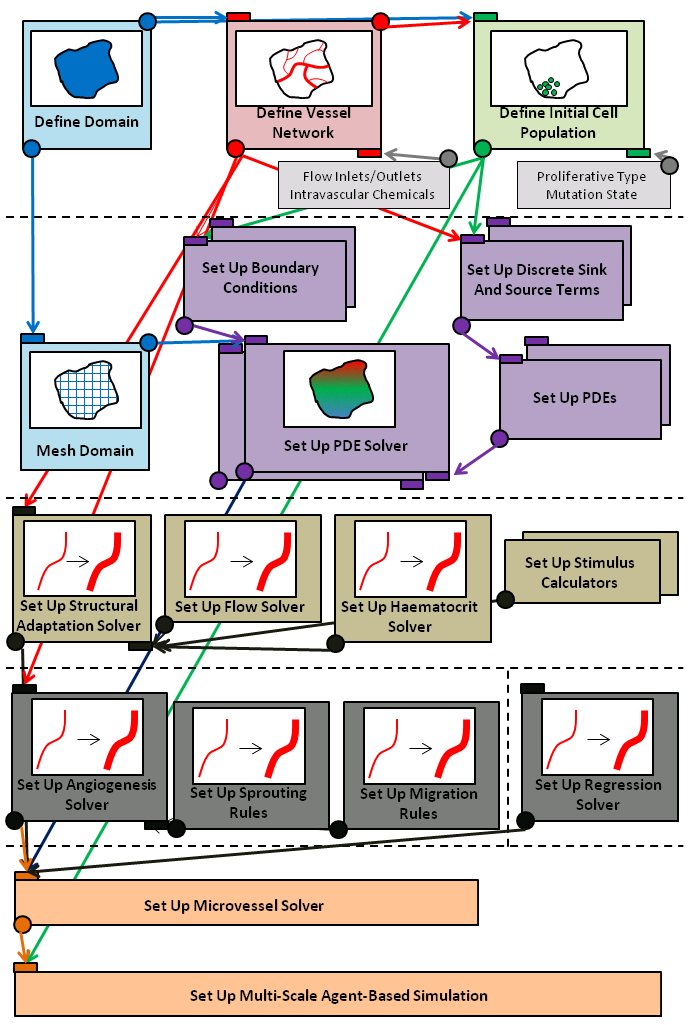
\includegraphics[width=0.9\textwidth]{Fig1.png}
\caption{{\bf An example of how a microvessel model can be composed using Microvessel Chaste.}
A schematic showing the composition of a vascular tumour growth model using Microvessel Chaste. The ability to compose a model from a collection of sub-models and sub-sub-models is noted.}
\label{fig1}
\end{figure}

Fig~\ref{fig2} shows how the library can be used to \emph{solve} a problem of interest in vascular tumour modelling. Again, it is emphasised that the user need not follow the shown solution ordering, but can decide on ordering themselves by suitably over-riding `Solve()' and `Increment()' methods. It is noted that steps on the left-hand side of Fig~\ref{fig2} are already implemented as part of the agent-based cell modelling funcitonality in Chaste~\cite{Mirams2013}. The Microvessel Chaste library interacts with the cell based solution as a plug-in (called a `SimulationModifier') in Chaste, by modifying the contents of a cell population once per time step. This loose coupling gives some flexibility in model compposition, in that Microvessel Chaste can remain reasonably agnostic regarding the details of the cell solution procedure. However, since the `Microvessel Solver' has direct access to a cell population (via a pointer), as shown in Fig~\ref{fig1}, there is still scope for implementing detailed cell-vessel interactions if needed. In the example problem shown in Fig~\ref{fig2} vessels interact with (non-vessel) cells only via their shared influence on the solutions of chemical transport problems. Cell birth, death and cell-cycle progression can be affected by the PDE solution, which is sampled by each cell during the `CellDataUpdate' step. More detailed interactions such as cell-vessel spatial occlusion, or forming vessels from collections of discrete cells are also implemented in the library.

% Place figure captions after the first paragraph in which they are cited.
\begin{figure}[!h]
\centering
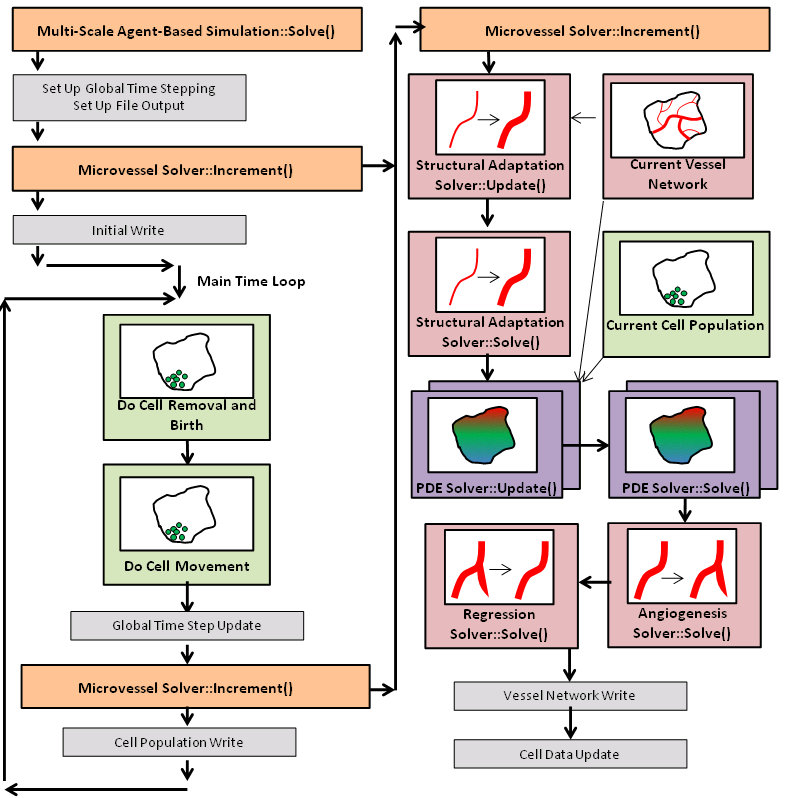
\includegraphics[width=0.8\textwidth]{Fig2.png}
\caption{{\bf An example of how a microvessel model can be solved using Microvessel Chaste.}
A schematic showing the solution of a vascular tumour growth model using Microvessel Chaste. It is noted that solution ordering can be readily changed by the user.}
\label{fig2}
\end{figure}

\subsection*{Code Layout And Design}

The components of the library are as follows:

\begin{itemize}
	\item geometry -- code for generating and describing 2D and 3D geometries using piece-wise linear complex (PLC) descriptions for direct use in Triangle and Tetgen meshing software.
	\item mesh -- code for automated finite element meshing of 2D and 3D geometries and interpolation of vessel and cell locations onto meshes and regular grids. 
	\item ode -- ode models for cell-cycling in vascular tumour problems.
	\item pde -- descriptions and solvers for steady state linear and non-linear PDEs with discrete sinks and sources for vessels and cells. Solvers use finite differences, finite element methods and Green's function methods~\cite{Secomb2013} based on Boost uBLAS and PETSc for vector and matrix operations.
	\item population -- code for describing, reading, writing and generating vessel networks.
	\item simulation -- flow, structural adaptation and angiogenesis solvers. Also code for managing integration of discrete vessel simulations with discrete cell populations from Chaste.
	\item utility -- dimensional analysis and collection of literature parameters of interest for tissue microvascualture simulations.	
\end{itemize}

As per the remainder of Chaste, object oriented programming, including templating in C++ are heavily utilized. Distinct from Chaste, shared pointers are used throughout to ease memory management. Input and output of vessel networks, regular grids, meshes and PDE results are in VTK (Paraview) format, which offer standard methods for visualization and post-processing. 

Python bindings are generated automatically using Py++ with a CASTXML backend. Automated generation is neccessary to account for the high degree of templating used in Chaste and Boost libraries and greatly eases code maintenance. A significant advantage of the provision of Python bindings for multi-scale agent-based models of this type is that compiled C++ classes can be overloaded in Python, without the need to re-compile the code. This gives allows for rapid and automatic model (or sub-model) generation based on mark-up language descriptions (for example, over-riding a cell cycle model based on an SBML description scraped from a web database).

During the development of the library it became apparent that there was potential for mis-use of units when quantities are passed into solvers which a modeller may not be familiar with, but would like to use none-the-less. As a simple example, oxygen consumption rates are often quoted as amount per cell per time (e.g. moles per second). If one is solving an oxygen reaction-diffusion PDE with oxygen partial pressure as the solution quantity (e.g. mmHg) it may be tempting to insert the literature oxygen consumption rate as a discrete sink term, per cell. A result will be produced, but the inputs have had dimensional incompatibilities. How did we convert from a partial pressure (mmHg) to an amount (moles)? A solubility term (mole per mmHg per metre cubed) is needed to convert partial pressure to concentration and a volume term to convert concentration to amount. Where does the volume term come from? It is from a volume integral over a point source (or delta function) with a value depending on the chosen numerical method for solving the PDE (e.g. the cube of the grid spacing in a 3D finite difference method). With compile-time dimensional analysis the code will not compile in C++ (or throw a type conversion exception in Python) if the user attempts to use incompatible dimensions, forcing a re-think regarding what they are actually modelling. A second advantage of the dimensional analysis functionality is that it allows automatic solver-specific non-dimensionalisation, which saves the user from performing this step and can help to ensure sufficient floating point accuracy.

% Results and Discussion can be combined.
\section*{Results}

In this section two example multi-scale agent-based problems are demonstrated, and are available for reproduction following wiki-based tutorials at \url{https://chaste.cs.ox.ac.uk/trac/wiki/PaperTutorials/Microvessel}.

\subsection*{A 2D Lattice Based Vascular Tumour Simulation}

The first example is a 2D lattice-based vascular tumour growth simulation following from Owen et al.~\cite{Owen2011}, but with some simplifications to reduce the computational expense of the tutorial. This example is to demonstrate the feasibility of replicating a well known vascular tumour growth simulation, which typifies many others in the literature (JG: add some model refs). It also demonstrates how the library interfaces with the functionality of well-known discrete cell modelling software, Chaste.

The problem is initialized with two large, parallel, counterflowing vessels, positioned on a regular lattice. A cellullar automaton based cell population is used to fill all lattice sites, with `cancer' cell types assigned to a central circular region and `normal' types to the remainder, as shon in Fig~\ref{fig3}. Due to their distance from the large vessels the tumour cells will become hypoxic and release growth factor (VEGF). This stimulates the growth of new vessels, which  migrate preferentially towards the tumour due to growth factor gradients. As shown in Fig~\ref{fig3}A the sprouts can merge if they meet. Vessel diameters can change over time due to flow induced stimuli, with low flow vessels eventually pruned. As shown in Fig~\ref{fig3}B, new vessels allow for increased oxygenation of the domain and eventual tumour growth. The tumour cells grow at the expense of immediately surrounding `normal' cells.

There are many potential additions to models of this type which have been explored in the literature, including ....

% Place figure captions after the first paragraph in which they are cited.
\begin{figure}[!h]
\centering
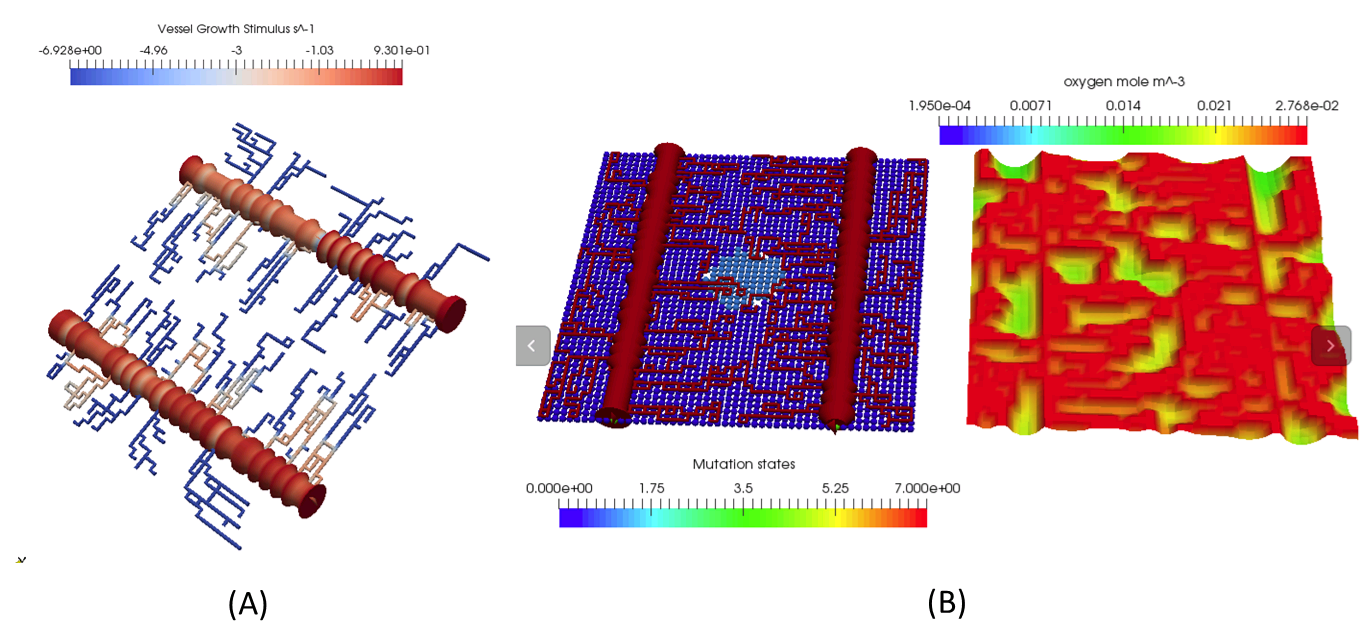
\includegraphics[width=0.99\textwidth]{Fig3.png}
\caption{{\bf An example of how a microvessel model can be solved using Microvessel Chaste.}
A schematic showing the solution of a vascular tumour growth model using Microvessel Chaste. It is noted that solution ordering can be readily changed by the user.}
\label{fig3}
\end{figure}

\subsection*{A 3D Off-Lattice Angiogenesis Simulation}

The second example is a 3D off-lattice simulation of angiogenesis on a curved surface. This example demonstrates more advanced features of the library in terms of 3D off-lattice angiogenesis and the solution of PDEs on arbitary domains. The application is in modelling the widely used corneal micropocket assay in the study of angiogenesis~\cite{Connor2015}. The authors are not aware of a previous study of angiogenesis on a curved surface in 3D. Discrete cells are excluded, which both reduces computational expense for the purposes of generating a tutorial and corresponds to a widely used modelling paradigm in which cells are treated as a continuum but vessels are modelled discretely~\cite{Secomb2013}.

% Place figure captions after the first paragraph in which they are cited.
\begin{figure}[!h]
\centering
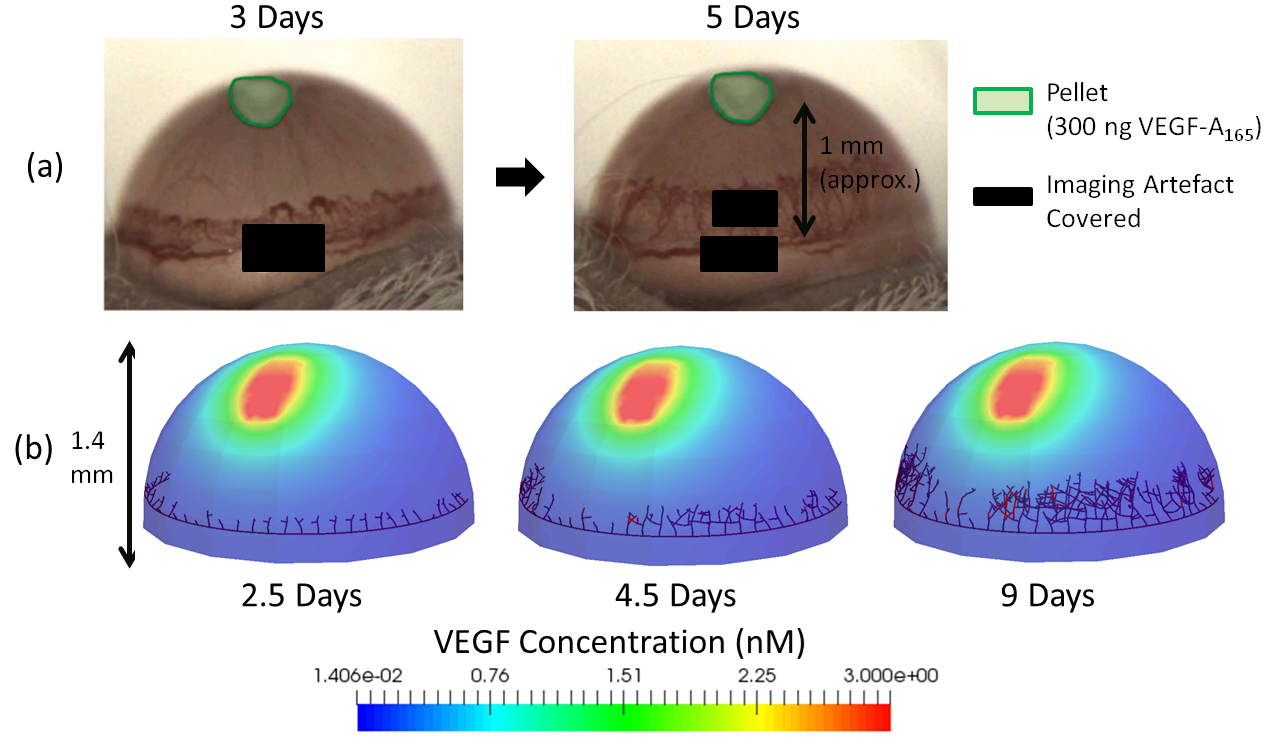
\includegraphics[width=0.6\textwidth]{Fig4.png}
\caption{{\bf An example of how a microvessel model can be solved using Microvessel Chaste.}
A schematic showing the solution of a vascular tumour growth model using Microvessel Chaste. It is noted that solution ordering can be readily changed by the user.}
\label{fig4}
\end{figure}

\section*{Availability and Future Directions}

Microvessel Chaste is available to download from the Chaste website  \url{https://chaste.cs.ox.ac.uk/trac/wiki/PaperTutorials/Microvessel}. The software is available under an open source Berkeley Software Distribution (BSD) licence. 

Additional functionality for semi-automated 2D and 3D image segmentation and meshing is under development to aid integration with experimental studies. Porting to Windows and Mac OS X are of interest, with future availbaility of Python packages for each likely. At present, alrogithms operate in serial only, however there is scope for distributed memory parallelisation for both C++ and Python interfaces. All PDE, Green's function and flow solvers are based on PETSc structures and vessel network components may be communicated using existing serialization functionality in Chaste~\cite{Harvey} or through VTK based serialization.

\subsection*{How to Become an Active Developer}

As discussed in Mirams et al.~\cite{Mirams2013}, contributions are welcome via the main Chaste website, which includes a developer wiki, mailing list details and the ability to open and comment on work tickets. A new git based version control system has recently been introduced for Chaste, which may further aid contribution in future.


\section*{Supporting Information}

% Include only the SI item label in the paragraph heading. Use the \nameref{label} command to cite SI items in the text.
\paragraph*{S1 Fig.}
\label{S1_Fig}
{\bf Bold the title sentence.} Add descriptive text after the title of the item (optional).

\paragraph*{S1 File.}
\label{S1_File}
{\bf Lorem Ipsum.}  Maecenas convallis mauris sit amet sem ultrices gravida. Etiam eget sapien nibh. Sed ac ipsum eget enim egestas ullamcorper nec euismod ligula. Curabitur fringilla pulvinar lectus consectetur pellentesque.

\section*{Acknowledgments}
Chaste team. Possibly contributors of vessel networks (e.g. Bostjan and co). Secomb for Greens Function code (our code has a re-write but maybe should also contact for general feedback).

\nolinenumbers

% Either type in your references using
% \begin{thebibliography}{}
% \bibitem{}
% Text
% \end{thebibliography}
%
% or
%
% Compile your BiBTeX database using our plos2015.bst
% style file and paste the contents of your .bbl file
% here.
% 
\begin{thebibliography}{10}

\bibitem{Mirams2013}
Mirams GR, Arthurs CJ, Bernabeu MO, Bordas R, Cooper J, Corrias A, Davit Y, Dunn S, Fletcher AG, Harvey DG, Marsh ME, Osborne JM, Pathmanathan P, Pitt-Francis J, Southern J, Zemzemi N, Gavaghan DJ.
\newblock {{C}haste: an open source C++ library for computational physiology and biology}.
\newblock PLoS Comp Bio. 2013 Jan;9(3):e1002970.

\bibitem{Cooper2015}
Cooper J, Spiteri RJ, Mirams GR.
\newblock {{C}ellular cardiac electrophysiology modeling with Chaste and CellML}.
\newblock Front Physiol. 2015 Jan;5:511.

\bibitem{Tetley2016}
Tetley RJ, Blanchard GB, Fletcher AG, Adams RJ, Sanson B.
\newblock {{U}nipolar distributions of junctional Myosin II identify cell stripe boundaries that drive cell intercalation throughout Drosophila axis extension}.
\newblock eLife. 2016 May;5:e12094.

\bibitem{Dunn2016}
Dunn SJ, Osborne JM, Appleton PL, Nathke I.
\newblock {{C}ombined changes in Wnt signaling response and contact inhibition induce altered proliferation in radiation-treated intestinal crypts}.
\newblock Mol Biol Cell. 2016 June;27(11):1863-1874.

\bibitem{Figueredo2013}
Figueredo GP, Joshi TV, Osborne J, Byrne HM, Owen MR.
\newblock {{O}n-lattice agent-based simulation of populations of cells within the open-source Chaste framework}.
\newblock Interface Focus. 2013 February;3(2):e20120081.

\bibitem{Owen2011}
Owen MR, Stamper J, Muthana M, Richardshon GW, Dobson J, Lewis CE, Byrne HM.
\newblock {{M}athematical modeling predicts synergistic antitumor effects of combining a macrophage-based, hypoxia-targeted gene therapy with chemotherapy}.
\newblock Cancer Res. 2015 April;71(8):2826-2837.

\bibitem{Swat2012}
Swat M, Thomas GL, Belmonte JM, Shirinifard A, Hmeljak D, Glazier JA.
\newblock {{M}ulti-scale modeling of tissues using CompuCell3D}.
\newblock Method in Cell Biol. 2012;110:325-366.

\bibitem{Sutterlin2013}
Sutterlin T, Kolb C, Dickhaus H, Jager D, Grabe N.
\newblock {{B}ridging the scales: semantic integration of quantitative SBML in graphical multi-cellular models and simulations with EPISIM and COPASI}.
\newblock Bioinformations. 2013 January;15(29):223-229.

\bibitem{Macklin2012}
Macklin P, Edgerton ME, Thompson AM, Cristini V.
\newblock {{P}atient-calibrated agent-based modelling of ductal carcinoma in situ (DCIS): From microscopic measurements to macroscopic predictions of clinical progression}.
\newblock J Theor Biol. 2012;301:122-140.

\bibitem{boost161}
Boost Development Team.
\newblock {{B}oost Units Reference Guide}.
\newblock Available: \url{http://www.boost.org/doc/libs/1_61_0/doc/html/boost_units.html}.

\bibitem{Secomb2013}
Secomb TW, Alberding JP, Hsu R, DeWhirst MW, Pries AR.
\newblock {{A}ngiogenesis: an adaptive dynamic biological patterning problem}.
\newblock PLoS Comp Bio. 2013;9(3):e1002983.

\bibitem{Anderson1998}
Anderson ARA, Chaplain MAJ.
\newblock {{C}ontinuous and discrete mathematical models of tumor-induced angiogenesis}.
\newblock Bullet Math Bio. 1998;60:857-900.

\bibitem{Frieboes2007}
Frieboes HB, Lowengrub JS, Wise S, Zheng X, Macklin P, Bearer E, Cristini V.
\newblock {{C}omputer simulation of glioma growth and morphology}.
\newblock Neuroimage. 2007;37(Supl 1):S59-S70.

\bibitem{Shirinifard2009}
Shirinifard A, Scott Gens J, Zaitlen L, Poplawski J, Swat M, Glazier JA.
\newblock {{3}D multi-cell simulation of tumor growth and angiogenesis}.
\newblock PLoS One. 2009;4(10):e7190.

\bibitem{Welter2013}
Welter M, Rieger H.
\newblock {{I}nterstitial fluid flow and drug delivery in vascularized tumors: a computational model}.
\newblock PLoS One. 2013;8(8):e70395.

\bibitem{Alarcon2005}
Alarcon T, Byrne HM, Maini PK.
\newblock {{A} multiple scale model for tumor growth}.
\newblock Multiscale model simul. 2005;3(2):440-475.

\bibitem{Perfahl2011}
Perfahl H, Byrne HM, Chen T, Estrella V, Alarcon T, Lapin A, Gatenby R, Gillies RJ, Llord MC, Maini PK, Reuss M, Owen MR.
\newblock {{M}ultiscale modelling of vascular tumour growth in 3D: the roles of domain size and boundary conditions}.
\newblock PLoS One. 2011 April;6(4):e14790.

\bibitem{Connor2015}
Connor AJ, Radoslaw P, Nowak EL, Thomas M, Hertig F, Hoert S, Quaiser T, Schocat E, Pitt-Francis J, Cooper J, Maini PK, Byrne HM.
\newblock {{A}n integrated approach to quantitative modelling in angiogenesis research}.
\newblock J R Soc Interface. 2015 August;12:e20150546.

\bibitem{Rieger2015}
Rieger H, Welter M.
\newblock {{I}ntegrative models of vascular remodeling during tumor growth}.
\newblock WIREs Syst Biol Med. 2015;7:113-129.

\bibitem{Connor2012}
Connor AJ, Cooper J, Byrne HM, Maini PK, McKeever S.
\newblock {{O}bject-oriented paradigms for modelling vascular tumor growth: a case study}.
\newblock In: The Fourth International Conference on Advances in Systems Simulation. Simul 2012. Iaria, Lisbon,74-83.

\bibitem{Tozer2004}
Tozer GM, Ameer-Berg SM, Baker J, Barber P, Hill SA, Hodgkiss R, Locke R, Prise V, Wilson I, Vojnovic B.
\newblock {{I}ntravital imaging of tumour vascular networks using multi-photon fluorescence microscopy}.
\newblock Advanced Drug Deliv Rev. 2005;57:135-152.

\bibitem{Grogan2016}
Grogan JA, Markelc B, Connor AJ, Muschel R, Pitt-Franics J, Maini PK, Byrne HM.
\newblock {{P}redicting the influence of microvascular structure on tumour response to radiotherapy}.
\newblock IEEE Trans Biomed Eng 2016;In Press,DOI:10.1109/TBME.2016.2606563.

\bibitem{bib2}
Ohno S.
\newblock Evolution by gene duplication.
\newblock London: George Alien \& Unwin Ltd. Berlin, Heidelberg and New York:
  Springer-Verlag.; 1970.

\bibitem{bib3}
Magwire MM, Bayer F, Webster CL, Cao C, Jiggins FM.
\newblock {{S}uccessive increases in the resistance of {D}rosophila to viral
  infection through a transposon insertion followed by a {D}uplication}.
\newblock PLoS Genet. 2011 Oct;7(10):e1002337.

\end{thebibliography}



\end{document}

